 \documentclass[11pt]{article} 
\usepackage[english]{babel}
\usepackage{pgfplots}
\usepackage{polynom}
\usepackage{hyperref}
\pgfplotsset{compat=1.6}

\pgfplotsset{soldot/.style={color=blue,only marks,mark=*}} \pgfplotsset{holdot/.style={color=blue,fill=white,only marks,mark=*}}

\usepackage[utf8]{inputenc}\usepackage{amsmath}
\usepackage{amssymb}
\usepackage{graphicx}
\usepackage[colorinlistoftodos]{todonotes}
\usepackage{listings,multicol}
\setlength{\oddsidemargin}{0.5cm} \setlength{\evensidemargin}{0cm}
\setlength{\textwidth}{16cm} \setlength{\textheight}{23cm}
\setlength{\topmargin}{-0.5cm}
\textheight 21.5cm
\newcommand{\function}[5]{
\begin{array}{cccl}
#1 :& #2 	& \longrightarrow 	& #3\\
	& #4	& \longmapsto		& #5
\end{array}
}

\usepackage[numbered,framed]{matlab-prettifier}
\lstMakeShortInline"
\lstset{
  style              = Matlab-editor,
  %basicstyle         = \mlttfamily,
  escapechar         = ",
  mlshowsectionrules = true,
}

\begin{document}

\title{T1 V2 NUMERICO 521230 UDEC}

\begin{minipage}{0.12\textwidth}

\includegraphics[width=\textwidth]{logoudec.eps}
\end{minipage}
\hspace{5mm}
\begin{minipage}{0.9\textwidth}
UNIVERSIDAD DE CONCEPCION\\
{\small\small\bf 
FACULTAD DE CIENCIAS\\ 
FISICAS Y MATEMATICAS}\\
DEPARTAMENTO DE INGENIERIA MATEMATICA\\
\rule{0.66\textwidth}{.5pt} Franco A. Milanese
\end{minipage}

\vspace{0.5cm}
\centerline{\bf Test I (521230)}
\begin{center}
 \begin{tabular}{p{0.7\textwidth}p{0.3\textwidth}}
	\textbf{Nombre:}   &\textbf{Carrera:}\\
	\textbf{Profesor:} & \textbf{ RUT:}
 \end{tabular}
 \\
 \vspace{0.2cm}
 \begin{tabular}{||p{2cm}|p{2cm}||p{2cm}||}
 \hline
 Pregunta 1 &  Pregunta 2 &     Total\\
 \hline

  \vspace{1.5cm} & &       \\
 \hline
 \end{tabular}
 \end{center}
 Enviar documentos solicitados en el formato solicitado a 
 %\textbf{veranonumerico@gmail.com}.

\begin{enumerate}
\item (40 pt) Cree una funci\'on de Matlab llamada \texttt{mimatriz()} que tenga como entrada un n\'umero natural $n$ y retorne una matriz de la forma
$$
\begin{bmatrix}
1 		& 2 		&  0 		& 0 		& 0 	&\cdots 	&n   \\
-2 		& 1 		& 2 		& 0 		& 0 	&\cdots 	&n+1 \\
0		&-2 		& 1 		& 2  		& 0 	&\cdots 	&n+2 \\
\vdots 	& \vdots 	& \ddots 	& \ddots 	& \ddots&			& \vdots \\
0		& 0			&0			& 0			&-2		& 1 		&2n-2\\
n		& n+1		& n+2 		& n+2		&  \cdots	&2n-2	& 2n-1
\end{bmatrix}_{n\times n}.
$$

\begin{enumerate}
	\item Estime para una n\'umero grande $n\in\mathbb{N}$ cuantos ceros tienen de las matrices de la estructura anterior
    \item En un rutero llamado \texttt{sistema.m}, resuelva mediante el método LU, utilizando el comando \texttt{lu()}, el sistema de matriz de coeficientes \texttt{mimatriz(6)} y vector del lado derecho $\begin{bmatrix} 1 & 2 & \cdots & 10\end{bmatrix}^T$   
    \item Determine si el comando \texttt{lu()} anterior utiliz\'o o no pivoteo parcial.
    
    \item Calcule la norma infinito de \texttt{mimatriz(10)}.
\end{enumerate}
Adjunte la funci\'on \texttt{mimatriz.m} y el fichero \texttt{sistema.m}.

 \textbf{Respuestas:} 
 La funci\'on \texttt{mimatriz()} debe tener instrucciones similares a
 
 \begin{minipage}{0.8\textwidth}
\begin{lstlisting}
function M=mimatriz(n)
M=diag(ones(1,n))+[zeros(n-1,1),diag(2*ones(1,n-1));zeros(1,n)]+[zeros(1,n);diag(-2*ones(1,n-1)),zeros(n-1,1)];
M(:,end)=(n:(2*n-1))';
M(end,:)=n:(2*n-1);
end
\end{lstlisting}
\end{minipage}
\hfill \fbox{20pt}
 
\begin{enumerate}
	\item Contamos las posiciones no nulas de esta estructura de matrices
  $$
  \begin{array}{rcl}
  N_{ceros}	= &\{\text{Total de componentes}\} &-\{\text{Componentes no nulas}\}\\
  			= & n^2	&-(2n+(n-1)+2(n-1)+n)\\
            = & n^2 -6n-3
 \end{array} \quad \fbox{5pt}
  $$
  \item El rutero \texttt{sistema.m} debe contener las instrucciones
  
\begin{minipage}{0.8\textwidth}
\begin{lstlisting}
  clear all;
[L,U,P]=lu(mimatriz(10));
y=(P*L)\[1:10]';
x=U\y
\end{lstlisting}
\end{minipage}
\hfill \fbox{5pt}

\item De donde se observa que el comando \texttt{lu()} de Matlab si utiliz\'o pivoteo parcial, puesto $P$ es una permutaci\'on de la identidad. \hfill \fbox{5pt}

\item Se puede demostrar o calcular con el comando \texttt{norm()} y su valor es $145$. \hfill \fbox{5pt}
\end{enumerate}

\item (20 pt) Considere la funci\'on
$$
\begin{array}{crcl}
f:	&[-10,4] & \longrightarrow 	& \mathbb{R} \\
	& x		& \longmapsto		& \begin{cases}
    								x^2+1   & \text{, si } x>0 \\
                                    2x+1	& \text{, si } x\leq 0
    								\end{cases}.
\end{array}
$$
En una misma figura grafique las funciones dadas por $f(x)$, $f(x+2)$, $f(cos(x))$ y $f(f(f(x)))$. Grabe esta im\'agen como \texttt{funciones2.jpg}. Adjunto al correo la imagen \texttt{funciones2.jpg} y todo rutero o funci\'on necesario para generarla.

 \textbf{Desarrollo:} Utilizando una funci\'on de matlab dada por
\begin{lstlisting}
function y=funcion(x)
y=(x.^2+1).*(x>0)+(2*x+1).*(x<=0)
end
\end{lstlisting}
y con el rutero

\begin{minipage}{0.8\textwidth}
\begin{lstlisting}
x=-10:0.1:4;
subplot(2,2,1)
plot(x,funcion(x));
subplot(2,2,2)
plot(x,funcion(x+2));
subplot(2,2,3)
plot(x,funcion(cos(x)));
subplot(2,2,4)
plot(x,funcion(funcion(funcion(x))));
\end{lstlisting}
\end{minipage}
 \fbox{10pt}
 
se crea la gr\'afica solicitada
\begin{center}
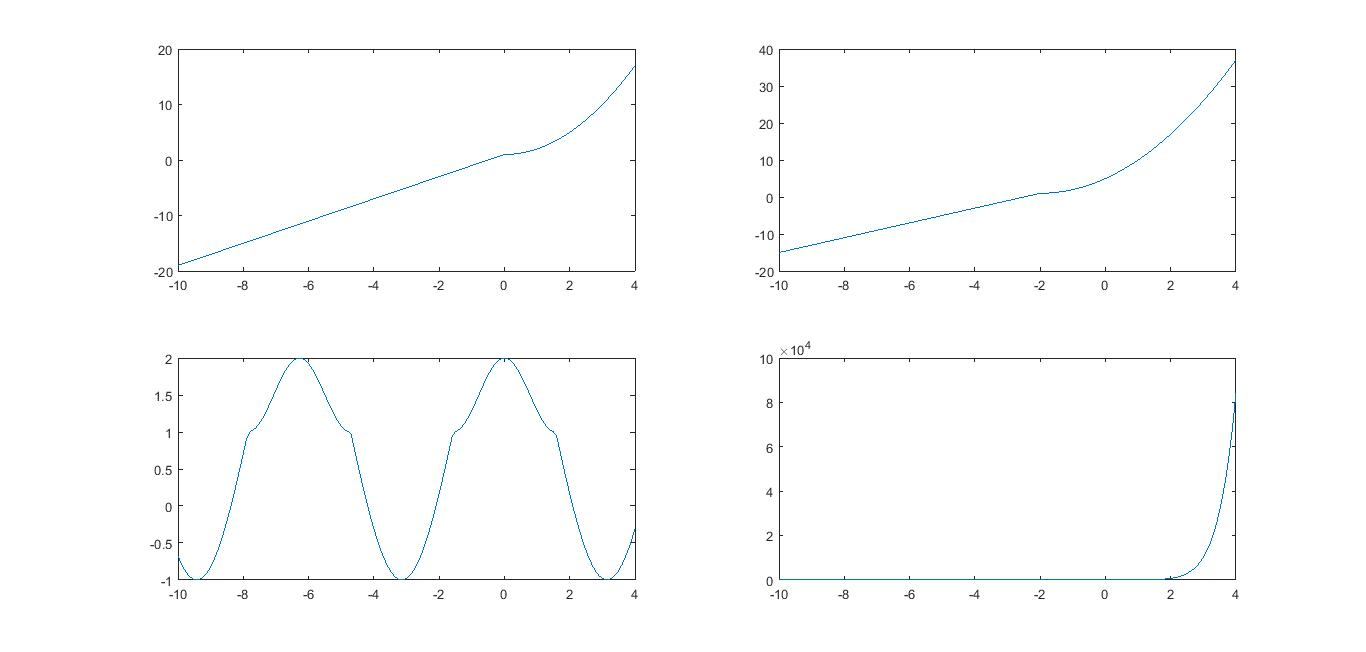
\includegraphics[width=0.7\textwidth]{funciones.jpg} 
\fbox{10 pt}
\end{center}

\end{enumerate}
\end{document}  